\section{Zentralitätsindizes}
\label{sec:centralities}

Ein Zentralitätsindex ist ein Maß, das intuitiv die Wichtigkeit eines Knoten oder einer Kante in einem Graphen wiedergibt. Betrachtet man den Graphen in Abbildung \ref{fig:randomGraph} als Straßennetzwerk, welches verschiedene Knotenpunkte miteinander verbindet und möchte herausfinden, welcher Knotenpunkt der am meisten belastete ist, kann dies durch ein Zentralitätsmaß erfasst werden. Ein Zentralitätsmaß weist jedem Knoten einen Wert zu, der die Wichtigkeit dieses Knoten widerspiegelt. So ist in der Abbildung der Knoten $F$ augenscheinlich der Knoten, der am meisten belastet wird. Zählt man nun für jeden Knoten die Anzahl der Kanten und benutzt den ermittelten Wert als Zentralitätsmaß, ergeben sich die Zentralitätswerte in Abbildung \ref{fig:randomGraphCentrality}. Das Zentralitätsmaß gibt das Erwartete wieder, da dem Knoten $F$ der größte Wert (5) zugewiesen wird. 

\begin{figure}[ht]
\centering
  \subfigure[Straßennetzwerk]{
    \begin{pspicture}(0,0)(5,4)

\cnode[fillstyle=solid, fillcolor=white](0,1){0.3}{B}
\cnode[fillstyle=solid, fillcolor=white](0,2.5){0.3}{A}

\cnode[fillstyle=solid, fillcolor=white](1,1){0.3}{E}
\cnode[fillstyle=solid, fillcolor=white](1,2){0.3}{D}
\cnode[fillstyle=solid, fillcolor=white](1,3){0.3}{C}

\cnode[fillstyle=solid, fillcolor=grey](2.5,2){0.3}{F}

\cnode[fillstyle=solid, fillcolor=white](4,1){0.3}{H}
\cnode[fillstyle=solid, fillcolor=white](4,3){0.3}{G}

\ncline{A}{C}
\ncline{A}{D}
\ncline{B}{E}

\ncline{C}{F}
\ncarc{C}{G}
\ncline{D}{F}
\ncline{E}{F}

\ncline{F}{H}
\ncline{F}{G}

\rput(0,1){$B$}
\rput(0,2.5){$A$}

\rput(1,1){$E$}
\rput(1,2){$D$}
\rput(1,3){$C$}

\rput(2.5,2){$F$}

\rput(4,1){$H$}
\rput(4,3){$G$}

\end{pspicture}

    \label{fig:randomGraph}
  }
  \subfigure[Straßennetzwerk mit Zentralitäten]{
    \begin{pspicture}(0,0)(5,4)

\cnode[fillstyle=solid, fillcolor=white](0,1){0.3}{B}
\cnode[fillstyle=solid, fillcolor=white](0,2.5){0.3}{A}

\cnode[fillstyle=solid, fillcolor=white](1,1){0.3}{E}
\cnode[fillstyle=solid, fillcolor=white](1,2){0.3}{D}
\cnode[fillstyle=solid, fillcolor=white](1,3){0.3}{C}

\cnode[fillstyle=solid, fillcolor=grey](2.5,2){0.3}{F}

\cnode[fillstyle=solid, fillcolor=white](4,1){0.3}{H}
\cnode[fillstyle=solid, fillcolor=white](4,3){0.3}{G}

\ncline{A}{C}
\ncline{A}{D}
\ncline{B}{E}

\ncline{C}{F}
\ncarc{C}{G}
\ncline{D}{F}
\ncline{E}{F}

\ncline{F}{H}
\ncline{F}{G}

\rput(0,1){1}
\rput(0,2.5){2}

\rput(1,1){2}
\rput(1,2){2}
\rput(1,3){3}

\rput(2.5,2){5}

\rput(4,1){1}
\rput(4,3){2}

\end{pspicture}

    \label{fig:randomGraphCentrality}
  }

\caption{Zentralitäten in einem Graphen}
\end{figure}

Es gibt noch viele anderen Zentralitätsmaße, die verschiedene Aspekte betrachten. Im Folgenden werden einige der für die Arbeit geeignet erscheinenden Zentralitätsmaße definiert und untersucht. Dazu benötigen wir zunächst einige wichtige Definitionen aus der Graphentheorie. 

\paragraph{Definition:} Ein Graph $G$ ist ein Tripel $(V,E,\omega)$, wobei $V=\lbrace v_1,\ldots,v_n\rbrace$ eine Menge von Knoten ist, $E=\lbrace e_1,\ldots,e_m \rbrace$ eine Menge von Kanten und $\omega: E \rightarrow \mathbb{R}$ eine Funktion, die jeder Kante $e \in E$ eine reelle Zahl zuordnet. 

Es kann zwischen gerichteten Graphen und ungerichteten Graphen unterschieden werden. Im ungerichteten Fall gilt
\[
E \subseteq \left\lbrace \{v,u\} | v,u \in V \right\rbrace \text{,}
\]
d.h. die Kante $\lbrace u,v \rbrace$ ist dieselbe wie $\lbrace v,u \rbrace$, da die Kanten als Mengen betrachtet werden und diese nicht sortiert sind. Im gerichteten Fall gilt
\[
E \subseteq \left\lbrace (u,v) | u,v \in V\right\rbrace \text{,}
\]
hier wird zwischen $(u,v) \in E$ und $(v,u) \in E$ unterschieden, da Paare sortiert sind.

Der Grad eines Knoten wird durch die Anzahl der eingehenden Kanten bzw. der ausgehenden Kanten bestimmt. Es ist $o(v)$ die Menge der ausgehenden Kanten eines Knoten $v$. Analog ist $i(v)$ die Menge der eingehenden Kanten. Im ungerichteten Fall gilt $o(v) = i(v)$. 

Ein Pfad $\pi$ ist definiert als eine Folge von Knoten $(v_1,\ldots,v_i,\ldots,v_n)$, wobei für alle $i,j \in \{1,\ldots,n\}$ gilt, dass $v_i \neq v_j$ falls $i \neq j$.

Die Distanz zwischen zwei Knoten $u$,$v$ wird mit $d(u,v)$ bezeichnet. Die Distanz zwischen zwei Knoten wird als die Summe der Gewichte auf dem Pfad von $u$ nach $v$ definiert. Im Falle, dass kein Pfad von $u$ nach $v$ existiert, gilt $d(u,v) = \infty$ und es gilt $d(u,u) = 0$. 

Eine formale Definition für Zentralitätsindizes wurde bis jetzt nicht aufgestellt. In \citet{Brandes2005} wird versucht, eine formalen Definition anzugeben. Dazu wird ein Zentralitätsindex als struktureller Index aufgefasst, der eine Halbordnung auf die Knoten bzw. Kanten des Graphen induziert. 

\paragraph{Definition:} Seien $\graph = (\vertexSet_\graph,\edgeSet_\graph)$ und $H=(\vertexSet_H,\edgeSet_H)$ gewichtete Graphen und $\Phi$ der Isomorphismus zwischen $G$ und $H$. Es bezeichne $X$ die Knotenmenge $\vertexSet_\graph$ bzw. die Kantenmenge $\edgeSet_\graph$. Dann ist $s$ ein struktureller Index genau dann, wenn $\forall x \in X: \graph \simeq H \Rightarrow s_\graph(x) = s_H(\Phi(x))$

Ein Zentralitätsindex muss ein struktureller Index sein, wobei nicht jeder strukturelle Index ein Zentralitätsindex ist. Durch die induzierte Halbordnung können wir Aussagen bzgl. eines Zentralitätsindex $\centrality{X}$ treffen, wie $x \in \vertexSet$ ist mindestens so zentral wie $y \in \vertexSet$ wenn $\centrality{X}(x) \geq \centrality{X}(y)$.

Für die einzelnen Klassen der Zentralitätsindizes wird in \citet{Brandes2005} versucht, eine axiomatische Definition herzuleiten. Diese hier wiederzugeben, würde den Fokus der Diplomarbeit verlassen. 

\subsection{Degree-Zentralität}
\label{subsec:degreecentrality}
Degree-Zentralität ist die einfachste Art der Zentralität. Die Zentralität der einzelnen Knoten wird anhand der Anzahl der ein- und ausgehenden Kanten bestimmt. 
Für gerichtete Graphen kann zwischen eingehenden und ausgehenden Kanten unterschieden werden. So ist die eingehende Degree-Zentralität definiert als \[\centrality{iD}(v) := |i(v)|\] 
und die ausgehende Degree-Zentralität als 
\[\centrality{oD}(v) := |o(v)|\] 
definiert. Im ungerichteten Fall gilt \[\centrality{D}(v) := |o(v)| \mbox{ oder } \centrality{D}(v) := |i(v)| \mbox{.}\]

Ein weiterer Zentralitätsindex bezieht zusätzlich zur Anzahl der Kanten noch die Gewichtung der Kanten mit ein. Die Shaffer-Zentralität $\centrality{SH}$ eines Knoten $v$ ist die Wurzel der Summe der quadrierten Gewichte der ein- bzw. ausgehenden Kanten. 
\[
\centrality{oSH}(v) = \sqrt{\sum_{u \in o(v)} \edgeWeight{(v,u)}^2 } \mbox{ bzw. } \centrality{iSH}(v) = \sqrt{\sum_{u \in i(v)} \edgeWeight{(u,v)}^2 }
\]

Der Vorteil der Degree-Zentralität Indizes ist die Unabhängigkeit von der Struktur des Graphen. Auch wenn der Graph nicht vollständig verbunden ist, können alle Knoten bewertet werden. Dies ist möglich, da die Knoten nur lokal betrachtet werden und die globale Struktur des Graphen außer Acht gelassen wird. Das kann je nach Anwendung ausreichend sein. Betrachtet man jedoch zum Beispiel, das Problem eine industrielle Anlage möglichst nah an allen Zulieferern aufzustellen, muss man die globale Struktur des Graphen berücksichtigen. Dazu eignen sich die folgenden Indizes besser. 

\subsection{Distanz}

Distanzbasierte Zentralitätsindizes berechnen die Zentralität anhand der Distanz zwischen den Knoten im Graphen. Bei distanzbasierten Zentralitäten geht es oft darum, eine öffentliche Einrichtungen in einem bestehenden Straßennetz zu platzieren, so dass bestimmte Kriterien erfüllt sind. 

\subsubsection{Eccentricity-Zentralität}
Ein Anwendungsbeispiel für die Eccentricity-Zentralität ist es, ein Krankenhaus zu platzieren, so dass die maximale Distanz zu allen Haushalten minimiert wird. Hierzu kann man das Exzentrizität-Zentralitätsmaß nutzen. Dieser Index berechnet, inwieweit ein Knoten im ``Inneren'' des Graphen liegt und bestimmt die Zentralität anhand der Exzentrizität der Knoten. Die Exzentrizität $e(v)$ eines Knoten $v$ ist definiert als der längste Pfad zu allen anderen Knoten $u$. D.h. $e(v) := max\lbrace d(u,v) | u \in V\rbrace$. Knoten, die in wenigen Schritten alle anderen Knoten erreichen können und im ``Inneren'' des Graphen liegen, sind somit zentraler als solche die weiter ``außen'' liegen. Die Eccentricity-Zentralität wird als die reziproke Exzentrizität definiert: 
\[\centrality{E}(v) := \frac{1}{e(v)}\]

Die Eccentricity-Zentralität in der obigen Formulierung weist die Schwäche auf, dass sie nur auf ungerichteten und zusammenhängenden Graphen definiert ist. Ist der Graph gerichtet oder nicht zusammenhängend kann es passieren, dass zwei Knoten nicht verbunden sind. Da für zwei Knoten $u,v$, die nicht verbunden sind, gilt, dass $d(v,u) = \infty$, ergibt die Exzentrizität $e(v) = \infty$ für alle Knoten $v$. Daraus folgt, dass die Zentralität $\centrality{E}$ nicht mehr definiert ist.

\subsubsection{Closeness-Zentralität}

Als Beispiel betrachte man das Problem einen Supermarkt zu bauen, so dass die totale Entfernung zu allen möglichen Kunden minimiert wird. Die Closeness-Zentralität kann bei der Lösung dieses Problem helfen. Sie wird als die Summe der Abstände zu allen anderen Knoten des Graphen definiert. Knoten mit einem niedrigen Closeness-Wert sind von allen anderen Knoten leichter erreichbar als Knoten mit einem hohen Wert. Entsprechend sind Knoten mit einem niedrigen Closenesswert zentraler als solche mit hohem Wert. Die Closeness-Zentralität wird dementsprechend analog zur Eccentricity-Zentralität definiert. Als reziproker Wert der Summe aller Pfade von $v$ zu allen anderen Knoten $u$.
\[c_C(v) := \frac{1}{\sum_{u \in V}d(u,v)}\mbox{.}\]
Der Supermarkt muss also an dem Knoten aufgestellt werden, der die höchste Closeness-Zentrali"-tät besitzt.

\subsubsection{Valente-Foreman-Closeness-Zentralität} 

Die Valente-Foreman-Closeness-Zentralität ist ein Abwandlung der Closeness-Zentralität. Sie ist definiert als 
\[
  c_R(v) := \frac{\sum_{u \in V}\Delta_G + 1 - d(v,u)}{n-1}
\] 
wobei $\Delta_G$ der Durchmesser des Graphen (der längste Pfad im Graphen) ist und $n := |V|$. Im Unterschied zur Closeness-Zentralität wird nicht der reziproke Wert der Closeness genommen, sondern die Distanz invertiert und so die entstehenden Werte gemittelt. 

Auch hier gilt, dass die Closeness-Zentralität und die Valente-Foreman-Closeness-Zentralität aus den gleichen Gründen wie die Eccentricity-Zentralität für nicht zusammenhängende oder Spezialfälle von gerichteten Graphen nicht definiert sind.

\subsection{Shortest-Path}

Shortest-Path Zentralitätsindizes für Knoten berechnen die Zentralität anhand der Anzahl der kürzesten Pfade, die durch einen Knoten führen. Betrachtet man wieder ein Straßennetz, in dem die Knoten Mautstationen repräsentieren und möchte wissen, durch welche Mautstation die meisten Fahrzeuge fahren, kann man Shortest-Path-Zentralitäten benutzen. Diese geben wieder, wie viel Arbeit ein Knoten leisten muss, bzw. wie viele Fahrzeuge durch die Mautstation geschleust werden. 

\subsubsection{Stress-Zentralität}

Die Stress-Zentralität misst, wie viel kürzeste Pfade durch einen Knoten im Graphen laufen. Zur Berechnung werden für einen Knoten $v$ die Anzahl der kürzesten Wege, die von einem Knoten $s$ zu einem Knoten $t$ führen, aufsummiert. Die Formel der Zentralität lautet: 
\[c_S(v) := \sum_{s \neq v \in V}\sum_{t \neq v \in V}\sigma_{st}(v)\]
 $\sigma_{st}(v)$ gibt die Anzahl der kürzesten Pfade von $s$ nach $t$ über $v$ an.

Dieser Index funktioniert für gerichtete und ungerichtete Graphen mit Kantengewichten. Definiert man $\sigma_{st}(v) = 0$, wenn es keinen Pfad von $s$ nach $t$ über $v$ gibt, dann funktioniert die Stress-Zentralität auch für nicht zusammenhängende Graphen bzw. für spezielle Konfigurationen von gerichteten Graphen.

\subsubsection{Betweenness -Zentralität}

Betweenness-Zentralität kann als eine Art normalisierte Stress-Zentralität betrachtet werden. Hier wird die Anzahl der kürzesten Pfade von $s$ nach $t$ über $v$ durch die Anzahl aller kürzesten Pfade von $s$ nach $t$ dividiert und somit relativiert. Die Formel ist analog zur Formel der Stress-Zentralität 
\[c_B(v) := \sum_{s \neq v \in V}\sum_{t \neq v \in V}\frac{\sigma_{st}(v)}{\sigma_{st}}\]
Hierbei bezeichnet $\sigma_{st}$ die Anzahl der kürzesten Pfade von $s$ nach $t$. Im Gegensatz zur Stress-Zentralität wird nicht die absolute Anzahl der kürzesten Pfade durch einen Knoten gezählt, sondern die relative Anzahl. So können Knoten, die eine hohe Last haben, besser bewertet werden (siehe \citep{Brandes2005} S. 30 Abb. 3.6).
Im Gegensatz zur Stress-Zentralität funktioniert die Betweenness-Zentralität nicht auf unzusammenhängenden Graphen. Auch hier gilt wieder: Sobald kein Pfad zwischen zwei Knoten $s,t \in \vertexSet$ existiert, ist die Betweenness-Zentralität nicht mehr definiert. 

\subsection{Feedback-Zentralitäten}

Die Feedback Zentralitäten wurden zuerst bei der Bewertung von Webseiten benutzt \citep{pagerank,hits}. Die Idee ist, dass eine Webseite hoch bewertet wird, wenn viele andere gut bewertete Webseiten auf diese verlinken. Die Bewertung bzw. die Zentralität wird an die benachbarten Seiten weitergegeben. So können Seiten, auf die zwar nicht oft verlinkt wird, trotzdem gut bewertet werden, wenn die wenigen verlinkenden Seiten eine hohe Bewertung aufweisen. Zusätzlich werden Seiten mit vielen eingehenden Links besser bewertet. 

\subsubsection{PageRank}
PageRank ist eine solche Feedback-Zentralität \citep{pagerank}. Die Zentralität eines Knoten wird anhand der Zentralitäten der benachbarten Knoten berechnet. Es gilt folgendes zu berechnen. 
\begin{equation}
\centrality{PR}(v) = d \sum_{u \in i(v)}\frac{\centrality{PR}(u)}{|o(u)|} + (1 - d)
\label{eq:prNonRecursiveFromula}
\end{equation}
Für jeden Knoten $v$ wird die Zentralität anhand der Summe der Zentralitäten der Knoten $u$, die auf $v$ zeigen, gewichtet mit der Anzahl der ausgehenden Kanten von $u$, berechnet. Fasst man nun die Zentralitäten aller Knoten $v_i,\ \ i \in \{1,\ldots,N\}$  in einem Vektor zusammen, so dass 
\[
\mathbf{\centrality{PR}} := (\centrality{PR}(v_1),\ldots,\centrality{PR}(v_N))
\] 
gilt, kann man die obige Formel auch in Matrixschreibweise darstellen. 
\begin{equation}
\mathbf{\centrality{PR}} = d\mathit{P}\mathbf{\centrality{PR}} + (1-d)\mathbf{1_N}
\label{eq:pageRank}
\end{equation}
Wobei die Übergangsmatrix $\mathit{P}$ definiert ist als 
\[
p_{ij} := \begin{cases}
\frac{1}{|o(j)|} & \text{wenn } (j,i) \in E \\
0 & \text{sonst}
\end{cases}
\text{.}
\]
Das rekursive Gleichungssystem in \ref{eq:pageRank} kann durch eine Jacobi-Iteration gelöst werden \citep{Brandes2005}. Mit den richtigen Werten initialisiert und mit $0 \leq d < 1$ konvergiert das Gleichungssystem gegen den gesuchten Wert $\mathbf{\centrality{PR}}^*$. Sei $\mathbf{\centrality{PR}}^0 := 1^N$ der Startwert für den Zentralitätsvektor $\mathbf{\centrality{PR}}$, dann ist 
\[
\mathbf{\centrality{PR}}^{i} = d\mathit{P}\mathbf{\centrality{PR}}^{i-1} + (1-d)\mathbf{1_N}
\]
und es gilt 
\[
\lim_{i \rightarrow \infty} \mathbf{\centrality{PR}}^i = \mathbf{\centrality{PR}}^* \text{.}
\]
Durch die Konstruktion der Übergangsmatrix $\mathit{P}$ wird die Gewichtung der Kanten nicht betrachtet und es wird nur die Struktur des Graphen und die Zentralität der benachbarten Knoten berücksichtigt. Verwendet man die Matrixschreibweise zur Berechnung der Zentralität, können auch nicht zusammenhängende Graphen betrachtet werden. So ist für den Graphen in Abbildung \ref{fig:disconnectedGrapPR} die Übergangsmatrix definiert als 
\[
\mathit{P} = 
\left(
\begin{array}{cc}
0 & 0 \\
0 & 0 \\
\end{array}
\right)
\]
und die Zentralitäten für $u$ und $v$ wären Null. Die rekursive Formel \ref{eq:prNonRecursiveFromula} wäre jedoch nicht mehr definiert, da durch Null geteilt würde.

\begin{figure}
\centering
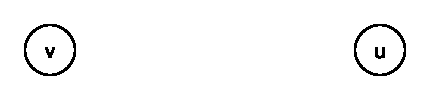
\includegraphics[scale=1]{images/content/02_fundamentals/disconnectedGraphPR} 
\caption{Nicht verbundener Graph}
\label{fig:disconnectedGrapPR}
\end{figure}

\subsubsection{Hits}
Hits ist wie PageRank zuerst zur Bewertung von Internetseiten verwendet worden \citep{hits}. Der Algorithmus kann jedoch auch als Zentralitätsmaß verwendet werden. Traditionell wird aus einem Grundstock von Webseiten, passend zu einer Anfrage, ein Graph erstellt, auf den dann Hits angewendet wird. Im Gegensatz zu PageRank berechnet Hits für jeden Knoten zwei Werte. Einmal den Authority-Wert, der angibt, wie gut der Knoten die Anfrage widerspiegelt. Dies wird anhand der Hub-Gewichte der Knoten, auf die die Authority zeigt, berechnet. Zweitens das Hub-Gewicht, welches angibt, auf wie viele wichtige Knoten verlinkt wird. Das Hub-Gewicht wird anhand der Authority-Gewichte der Knoten berechnet, auf die der Hub zeigt.

Mathematisch kann das Authority-Gewicht folgendermaßen berechnet werden
\begin{equation}
\centrality{H_a}(v_i) = \sum^n_{k=1}A^T_{ik}\centrality{H_h}(v_k)
\label{eq:rekAuth}
\end{equation}
und das Hub-Gewicht folgendermaßen
\begin{equation}
\centrality{H_h}(v_i) = \sum^n_{j=1}A_{ik}\centrality{H_a}(v_j) \text{.}
\label{eq:rekHub}
\end{equation}
Wobei $A$ die Adjazenzmatrix des Graphen ist, $\centrality{H_a}$ die Authority-Gewichtung und $\centrality{H_h}$ die Hub-Gewichtung. Substituiert man $\centrality{H_h}(v_k)$ mit $\centrality{H_a}(v_k)$ in Gleichung \ref{eq:rekAuth} und $\centrality{H_h}(v_k)$ mit $\centrality{H_a}(v_k)$ in Gleichung \ref{eq:rekHub}, erhält man die Formeln in Matrixschreibweise. So lässt sich die Authority-Gewichtung durch Gleichung \ref{eq:matrixAuth} ausdrücken und die Hub-Gewichtung durch Gleichung \ref{eq:matrixHub}. 
\begin{equation}
\mathbf{\centrality{H_a}} = (A^TA)\mathbf{\centrality{H_a}}
\label{eq:matrixAuth}
\end{equation}
\begin{equation}
\mathbf{\centrality{H_h}} = (AA^T)\mathbf{\centrality{H_h}}
\label{eq:matrixHub}
\end{equation}
Die $\mathbf{\centrality{H_a}}$ bzw. $\mathbf{\centrality{H_h}}$ bezeichnen dabei wieder die Vektoren der Zentralität. Als Zentralitätsindex kann, je nach Anwendung, sowohl die Authority-Gewichtung als auch die Hub-Gewichtung benutzt werden. Die Authority-Gewichtung eignet sich, wenn Knoten nach Anzahl der eingehenden Kanten und der Hubgewichtung der Knoten, die auf den Authority-Knoten zeigen, bewertet werden sollen. Die Hub-Gewichtung eignet sich, wenn Knoten nach Anzahl der ausgehenden Kanten und der Authority-Gewichtung der Knoten, auf die die Kanten zeigen, bewertet werden sollen.